\documentclass[12pt,a4paper]{article}

% Language setting
\usepackage[british]{babel}

% Set page size and margins
\usepackage[a4paper,top=2cm,bottom=2cm,left=2.5cm,right=2.5cm,marginparwidth=1.75cm]{geometry}

%----------- APA style references & citations (starting) ---
% Useful packages
%\usepackage[natbibapa]{apacite} % APA-style citations.

\usepackage[style=apa, backend=biber]{biblatex} % APA 7th edition style citations using biblatex
\addbibresource{references.bib} % Your .bib file

% Formatting DOI in APA-7 style
%\renewcommand{\doiprefix}{https://doi.org/}

% Add additional APA 7th edition requirements
\DeclareLanguageMapping{british}{british-apa} % Set language mapping
\DeclareFieldFormat[article]{volume}{\apanum{#1}} % Format volume number

% Modify 'and' to '&' in the bibliography
\renewcommand*{\finalnamedelim}{%
  \ifnumgreater{\value{liststop}}{2}{\finalandcomma}{}%
  \addspace\&\space}
  
%----------- APA style references & citations (ending) ---


\usepackage{amsmath}
\usepackage{graphicx}
\usepackage[colorlinks=true, allcolors=blue]{hyperref}
\usepackage{hyperref}
%\usepackage{orcidlink}
\usepackage[title]{appendix}
\usepackage{mathrsfs}
\usepackage{amsfonts}
\usepackage{booktabs} % For \toprule, \midrule, \botrule
\usepackage{caption}  % For \caption
\usepackage{threeparttable} % For table footnotes
\usepackage{algorithm}
\usepackage{algorithmicx}
\usepackage{algpseudocode}
\usepackage{listings}
\usepackage{enumitem}
\usepackage{chngcntr}
\usepackage{booktabs}
\usepackage{lipsum}
\usepackage{subcaption}
\usepackage{authblk}
\usepackage[T1]{fontenc}    % Font encoding
\usepackage{csquotes}       % Include csquotes
\usepackage{diagbox}


% Customize line spacing
\usepackage{setspace}
\onehalfspacing % 1.5 line spacing

% Redefine section and subsection numbering format
\usepackage{titlesec}
\titleformat{\section} % Redefine section numbering format
  {\normalfont\Large\bfseries}{\thesection.}{1em}{}
  
% Customize line numbering format to right-align line numbers
\usepackage{lineno} % Add the lineno package
\renewcommand\linenumberfont{\normalfont\scriptsize\sffamily\color{blue}}
\rightlinenumbers % Right-align line numbers

\linenumbers % Enable line numbering

% Define a new command for the fourth-level title.
\newcommand{\subsubsubsection}[1]{%
  \vspace{\baselineskip}% Add some space
  \noindent\textbf{#1\\}\quad% Adjust formatting as needed
}
% Change the position of the table caption above the table
\usepackage{float}   % for customizing caption position
\usepackage{caption} % for customizing caption format
\captionsetup[table]{position=top} % caption position for tables

% Define the unnumbered list
\makeatletter
\newenvironment{unlist}{%
  \begin{list}{}{%
    \setlength{\labelwidth}{0pt}%
    \setlength{\labelsep}{0pt}%
    \setlength{\leftmargin}{2em}%
    \setlength{\itemindent}{-2em}%
    \setlength{\topsep}{\medskipamount}%
    \setlength{\itemsep}{3pt}%
  }%
}{%
  \end{list}%
}
\makeatother

% Suppress the warning about \@parboxrestore
\pdfsuppresswarningpagegroup=1


%-------------------------------------------
% Paper Head
%-------------------------------------------
\title{Article title article title}

\author[1]{First Author}
\author[2]{Second Author}
\author[2]{Third Author}
\author[3]{Fourth Author}
\author[1,*]{Fifth Author}
\affil[1]{\small Department, Organization, Street, City, 100190, State, Country}
\affil[2]{Department, Organization, Street, City, 10587, State, Country}
\affil[3]{Department, Organization, Street, City, 610101, State, Country}
\affil[*]{Corresponding author: \texttt{user\_id@university.edu}}

\date{}  % Remove date

\begin{document}
\maketitle

\begin{abstract}
Abstracts must be able to stand alone and so cannot contain citations to the paper’s references, equations, etc. An abstract must consist of a single paragraph and be concise. Because of online formatting, abstracts must appear as plain as possible. Three to six keywords must be included. Each keyword should not exceed three words. %\lipsum[1]
\end{abstract}

\textbf{Keywords}: keyword1, keyword2, keyword3, keyword4, keyword5, keyword6.  

%-------------------------------------------
% Paper Body
%-------------------------------------------
%--- Section ---%
\section*{Nomenclature}

\begin{tabbing}
$T$\qquad \= Temperature (K)\\
$u_i$ \> Velocity in the x-direction (m/s)\\
$\tau_{ij}$ \> Shear stress (N/m2)\\
$\omega$ \> Specific turbulent dissipation rate (1/s)\\
$Y_\omega$ \> Dissipation of $\omega$
\end{tabbing}



%--- Section ---%
\section{Introduction}



%--- Section ---%
\section{Example of First Level Head - Section Head}\label{sec2}

\lipsum[4]

\lipsum[4]


\subsection{How to create sections and subsections}
Simply use the section and subsection commands, as in this example document! With Overleaf, all the formatting and numbering is handled automatically according to the template you've chosen. If you're using the Visual Editor, you can also create new sections and subsections via the buttons in the editor toolbar.

\subsection{This is an example of second level head - subsection head}\label{subsec1}
\lipsum[5]

\subsubsection{This is an example of third level head - subsubsection head}\label{subsubsec1}
\lipsum[6]

\subsubsubsection{This is an example of fourth level head - paragraph head}
\lipsum[7]


%--- Section ---%
\section{Example of First Level Head}\label{sec3}

\subsection{This is an example of second level head - subsection head}\label{subsec2}

\subsubsection{This is an example of third level head - subsubsection head}\label{subsubsec2}
\lipsum[8]

\subsubsubsection{This is an example of fourth level head - paragraph head}
\lipsum[9]


%--- Section ---%
\section{How to Include Equations}\label{sec4}

Equations in \LaTeX{} can either be inline or set as display equations. For
inline equations use the \verb+$...$+ commands. Eg: the equation
$H\psi = E \psi$ is written via the command \verb+$H \psi = E \psi$+.

For display equations (with auto generated equation numbers)
one can use the equation or eqnarray environments:
\begin{equation}
\|\tilde{X}(k)\|^2 \leq\frac{\sum\limits_{i=1}^{p}\left\|\tilde{Y}_i(k)\right\|^2+\sum\limits_{j=1}^{q}\left\|\tilde{Z}_j(k)\right\|^2 }{p+q},
\label{eq1}
\end{equation}
where
\begin{align}
D_\mu &=  \partial_\mu - ig \frac{\lambda^a}{2} A^a_\mu \nonumber \\
F^a_{\mu\nu} &= \partial_\mu A^a_\nu - \partial_\nu A^a_\mu + g f^{abc} A^b_\mu A^a_\nu
\label{eq2}
\end{align}
Notice the use of \verb+\nonumber+ in the align environment at the end
of each line, except the last, so as not to produce equation numbers on
lines where no equation numbers are required. The \verb+\label{}+ command
should only be used at the last line of an align environment where
\verb+\nonumber+ is not used.
\begin{equation}
Y_\infty = \left( \frac{m}{\textrm{GeV}} \right)^{-3}
    \left[ 1 + \frac{3 \ln(m/\textrm{GeV})}{15}
    + \frac{\ln(c_2/5)}{15} \right]
\label{eq3}
\end{equation}
The class file also supports the use of \verb+\mathbb{}+, \verb+\mathscr{}+ and
\verb+\mathcal{}+ commands. As such \verb+\mathbb{R}+, \verb+\mathscr{R}+
and \verb+\mathcal{R}+ produces $\mathbb{R}$, $\mathscr{R}$ and $\mathcal{R}$
respectively 
%(refer Subsubsection~\ref{subsubsec3}).

Equations must be provided as editable text, either in a Word or LaTeX source file. They should be numbered consecutively through the manuscript as shown in Equations \ref{eq1}, \ref{eq2} and \ref{eq3}. In APA style, when discussing numbered equations in the text, write out the word “Equation” and give the number. For example, you would write “see Equation \ref{eq1}.”
Use no punctuation after the equation if it appears at the end of a sentence; however, it is permissible (and may even be necessary) to place some form of punctuation after it (a comma or semi-colon, for example) if it appears in the middle of the sentence and is followed by text. In any case, maintain the coherence of all sentences with equations in them.


%--- Section ---%
\section{How to Include Tables}\label{sec5}

Use the table and tabular environments for basic tables --- see Tables~\ref{tab1} and \ref{tab2}, for example. Table \ref{tab1} is an sample figure including table footnotes. For more information, please see this help article on \href{https://www.overleaf.com/learn/latex/tables}{tables}. 

\begin{table}[!ht]
\caption{Sample table with footnotes\label{tab1}}
\begin{threeparttable}
\begin{tabular*}{\columnwidth}{@{\extracolsep\fill}llll@{\extracolsep\fill}}
\toprule
column 1 & column 2 & column 3 & column 4\\
\midrule
row 1 & data 1 & data 2 & data 3 \\
row 2 & data 4 & data 5\tnote{1} & data 6 \\
row 3 & data 7 & data 8 & data 9\tnote{2} \\
\bottomrule
\end{tabular*}
\begin{tablenotes}
\item Source: This is an example of table footnote. This is an example of table footnote. This is an example of table footnote. This is an example of table footnote. This is an example of table footnote.
\item[1] Example of a first table footnote.
\item[2] Example of a second table footnote.
\end{tablenotes}
\end{threeparttable}
\end{table}

\begin{table*}[!ht]
\caption{Example of a lengthy table which is set to full textwidth.\label{tab2}}
\tabcolsep=0pt
\begin{threeparttable}
\begin{tabular*}{\textwidth}{@{\extracolsep{\fill}}lcccccc@{\extracolsep{\fill}}}
\toprule
& \multicolumn{3}{c}{Element 1\tnote{1}} & \multicolumn{3}{c}{Element 2\tnote{2}} \\
\cmidrule(lr){2-4}\cmidrule(lr){5-7}
Project & Energy & $\sigma_{\mathrm{calc}}$ & $\sigma_{\mathrm{expt}}$ & Energy & $\sigma_{\mathrm{calc}}$ & $\sigma_{\mathrm{expt}}$ \\
\midrule
Element 3 & 990 A & 1168 & $1547\pm12$ & 780 A & 1166 & $1239\pm100$ \\
Element 4 & 500 A & 961 & $922\pm10$ & 900 A & 1268 & $1092\pm40$ \\
\bottomrule
\end{tabular*}
\begin{tablenotes}
\item Note: This is an example of table footnote this is an example of table footnote this is an example of table footnote this is an example of~table footnote this is an example of table footnote.
\item[1] Example of a first table footnote.
\item[2] Example of a second table footnote.
\end{tablenotes}
\end{threeparttable}
\end{table*}


%--- Section ---%
\section{How to Include Figures}\label{sec6}

First you have to upload the image file from your computer using the upload link in the file-tree menu. Then use the includegraphics command to include it in your document. Use the figure environment and the caption command to add a number and a caption to your figure. See the code for Figure \ref{fig:cat1} in this section for an example. As shown in Figures \ref{fig:cat1} and \ref{fig:multi_figs}, the images should be single-page documents. 

Note that your figure will automatically be placed in the most appropriate place for it, given the surrounding text and taking into account other figures or tables that may be close by. You can find out more about adding images to your documents in this help article on \href{https://www.overleaf.com/learn/how-to/Including_images_on_Overleaf}{including images on Overleaf}.

\begin{figure}[!ht]
\centering
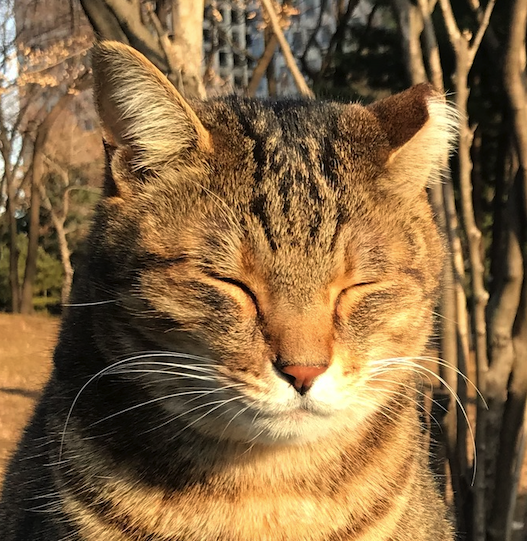
\includegraphics[width=0.4\linewidth]{figures/cat_momo_1.png}
\caption{\label{fig:cat1}This cat picture is located at the 'figures' folder.}
\end{figure}

\subsection{More information about figures}

As per display \LaTeX\ standards one has to use eps images for \verb+latex+ compilation and \verb+pdf/jpg/png+ images for
\verb+pdflatex+ compilation. This is one of the major differences between \verb+latex+
and \verb+pdflatex+. The images should be single-page documents. The command for inserting images
for \verb+latex+ and \verb+pdflatex+ can be generalized. The package used to insert images in \verb+latex/pdflatex+ is the
graphicx package. Figures can be inserted via the normal figure environment as shown in the below example:


\begin{figure}[!ht]
    \begin{subfigure}{0.3\textwidth}
        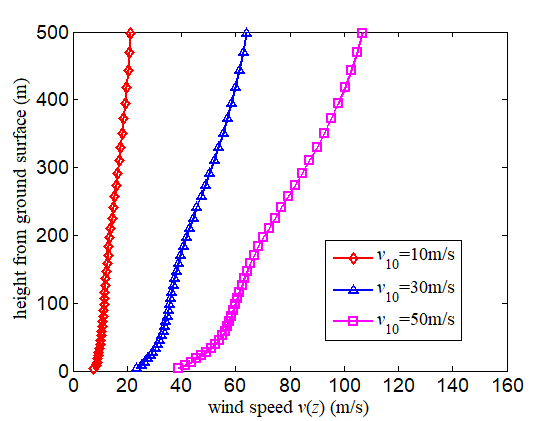
\includegraphics[width=\linewidth]{figures/fig_a.png}
        \caption{}
    \end{subfigure}
    \hfill
    \begin{subfigure}{0.3\textwidth}
        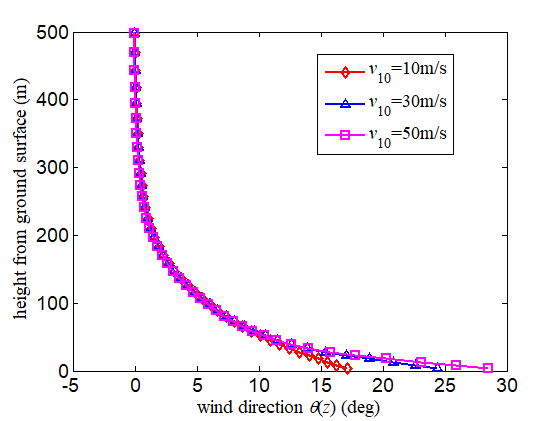
\includegraphics[width=\linewidth]{figures/fig_b.png}
        \caption{}
    \end{subfigure}
    \hfill
    \begin{subfigure}{0.3\textwidth}
        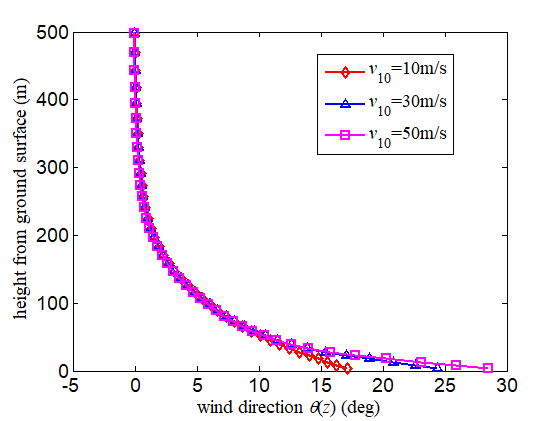
\includegraphics[width=\linewidth]{figures/fig_c.png}
        \caption{}
    \end{subfigure}
    \caption{Overall caption for the three figures: (a) caption for figure a, (b) caption for figure b, and (c) caption for figure c.}
    \label{fig:multi_figs}
\end{figure}


\begin{verbatim}
\begin{figure}[h]
        \centering\includegraphics{<eps-file>}
        \caption{<figure-caption>}
        \label{<figure-label>}
\end{figure}
\end{verbatim}


%--- Section ---%
\section{How to Include Algorithms, Program Codes, and Listings}\label{sec8}
Packages \verb+algorithm+, \verb+algorithmicx+, and \verb+algpseudocode+ are used for setting algorithms in latex.
For this, one has to use the below format:

\begin{verbatim}
\begin{algorithm}
\caption{<alg-caption>}\label{<alg-label>}
\begin{algorithmic}[1]
. . .
\end{algorithmic}
\end{algorithm}
\end{verbatim}

You may need to refer to the above-listed package documentation for more details before setting an \verb+algorithm+ environment.
To set program codes, one has to use the \verb+program+ package. We need to use the \verb+\begin{program}+ \verb+...+
\verb+\end{program}+ environment to set program codes.

\begin{algorithm}[!ht]
\caption{Calculate $y = x^n$}\label{algo1}
\begin{algorithmic}[1]
\Require $n \geq 0 \vee x \neq 0$
\Ensure $y = x^n$
\State $y \Leftarrow 1$
\If{$n < 0$}
        \State $X \Leftarrow 1 / x$
        \State $N \Leftarrow -n$
\Else
        \State $X \Leftarrow x$
        \State $N \Leftarrow n$
\EndIf
\While{$N \neq 0$}
        \If{$N$ is even}
            \State $X \Leftarrow X \times X$
            \State $N \Leftarrow N / 2$
        \Else[$N$ is odd]
            \State $y \Leftarrow y \times X$
            \State $N \Leftarrow N - 1$
        \EndIf
\EndWhile
\end{algorithmic}
\end{algorithm}

Similarly, for \verb+listings+, one has to use the \verb+listings+ package. To set environments similar to the \verb+verbatim+ environment, the \verb+\begin{lstlisting}+ \verb+... + \verb+\end{lstlisting}+ environment is used . Refer to the \verb+lstlisting+ package documentation for more details on this.

\begin{minipage}{\hsize}%
\lstset{language=Pascal}% Set your language (you can change the language for each code-block optionally)
\begin{lstlisting}[frame=single,framexleftmargin=-1pt,framexrightmargin=-17pt,framesep=12pt,linewidth=0.95\textwidth]
for i:=maxint to 0 do
begin
{ do nothing }
end;
Write('Case insensitive ');
Write('Pascal keywords.');
\end{lstlisting}
\end{minipage}


%--- Section ---%
\section{How to Include Lists}\label{sec7}

List in \LaTeX{} can be of three types: numbered, bulleted, and unnumbered. The ``enumerate'' environment produces a numbered list, the 
``itemize'' environment produces a bulleted list, and the ``unlist''
environment produces an unnumbered list.
In each environment, a new entry is added via the \verb+\item+ command.

\begin{enumerate}[label=\arabic*.]
\item This is the 1st item
\item Enumerate creates numbered lists, itemize creates bulleted lists, and unnumerate creates unnumbered lists.

\begin{enumerate}[label=\alph*.]
\item Second level numbered list. Enumerate creates numbered lists, itemize creates bulleted lists, and description creates unnumbered lists.
\item Second level numbered list. Enumerate creates numbered lists, itemize creates bulleted lists, and description creates unnumbered lists.

\begin{enumerate}[label=(\roman*)]
\item Third level numbered list. Enumerate creates numbered lists, itemize creates bulleted lists, and description creates unnumbered lists.
\item Third level numbered list. Enumerate creates numbered lists.
\end{enumerate}

\item Second level numbered list. Enumerate creates numbered lists, itemize creates bulleted lists, and description creates unnumbered lists.
\end{enumerate}

\item Numbered lists continue.
\end{enumerate}
Lists in \LaTeX{} can be of three types: enumerate, itemize, and description.
In each environment, a new entry is added via the \verb+\item+ command.

\begin{itemize}
\item First level bulleted list. This is the 1st item
\item First level bulleted list. Itemize creates bulleted lists, and description creates unnumbered lists.

\begin{itemize}
\item Second level dashed list. Itemize creates bulleted lists, and description creates unnumbered lists.
\item Second level dashed list. Itemize creates bulleted lists, and description creates unnumbered lists.
\end{itemize}

\item First level bulleted list. Bullet lists continue.
\end{itemize}

\noindent
Example of unnumbered list items:

\begin{unlist}
\item Sample unnumberd list text. Sample unnumberd list text. Sample unnumberd list text. Sample unnumberd list text. Sample unnumberd list text.

\item Sample unnumberd list text. Sample unnumberd list text. Sample unnumberd list text.

\item Sample unnumberd list text. Sample unnumberd list text. Sample unnumberd list text. Sample unnumberd list text. 
\end{unlist}


%--- Section ---%
\section{How to Add Citations and a References List}

You can simply upload a \verb|.bib| file containing your BibTeX entries, created with a tool such as JabRef. You can then cite entries from it, like this: \textcite{greenwade93}. Just remember to specify a bibliography style, as well as the filename of the \verb|.bib|. You can find a \href{https://www.overleaf.com/help/97-how-to-include-a-bibliography-using-bibtex}{video tutorial here} to learn more about BibTeX.

Here is an example citation when you want an author name like \textcite{collins2011a} to appear in the text. And here's how to do a parenthetic citation, when you want to mention a reference at the end of a sentence or part of a sentence \parencite{collins2013}. It is possible to cite multiple references at the same time \parencite{collins2011b,collins2016,lunn2007a,lunn2007b,ross2006,shannon1948}.

If you have an \href{https://www.overleaf.com/user/subscription/plans}{upgraded account}, you can also import your Mendeley or Zotero library directly as a \verb|.bib| file, via the upload menu in the file-tree.

\subsection{Citation in text}
Please ensure that every reference cited in the text is also present in the reference list (and vice versa). Citations in the text should follow the referencing style used by the American Psychological Association. You are referred to the Publication Manual of the American Psychological Association (APA), Seventh Edition, ISBN 978-1-4338-3215-4, copies of which may be ordered online. References in the Abstract should be avoided, but if essential, then cite the author(s) and year(s). Unpublished results and personal communications are not recommended in the reference list but may be mentioned in the text. If these references are included in the reference list, they should follow the standard reference style of the journal and should include a substitution of the publication date with either ‘Unpublished results’ or ‘Personal communication’. The citation of a reference as ‘in press’ implies that the item has been accepted for publication. 

An APA in-text citation includes only three items: the last name(s) of the author(s), the year the source was published, and sometimes the page or location of the information. More than one reference from the same author(s) in the same year must be identified by the letters ‘a’, ‘b’, ‘c’, etc., placed after the year of publication. The following paragraph shows examples of APA style of citations.

Here is an example citation when you want an author name like \textcite{collins2011a} to appear in the text. And here's how to do a parenthetic citation when you want to mention a reference at the end of a sentence or part of a sentence \parencite{collins2013}. It is possible to cite multiple references at the same time \parencite{collins2011b,collins2016,lunn2007a,lunn2007b,ross2006,shannon1948}.

The followings are examples of \verb+\textcite{...}+: \textcite{rahman2019centroidb}, \textcite{krizhevsky2012imagenet, horvath2018dna}, and \textcite{lecun2015deep, zhang2018fine, ravi2016deep}. Another example of \verb+\parencite{...}+: \parencite{bahdanau2014neural,imboden2018cardiorespiratory,motiian2017unified,murphy2012machine,ji20123d}.

\subsection{References}
The Reference Section, also called the Reference List or Cited Works List, is a list of the full-text details of the in-text citations that have been used in the main text. It includes information such as the name of the author(s), the year the source was published, the full title of the source, and the URL or page range. The Reference Section allows the reader to find the text easily and can be considered as the long-hand format of the in-text citation. It is found at the end of the piece of writing. The works in a reference section should be arranged first alphabetically and then further sorted chronologically if necessary.

\subsubsection{Web references}
As a minimum, the full URL and the date when the reference was last accessed should be given. Any further information, if known (DOI, author names, dates, reference to a source publication, etc.), should also be given. Web references can be listed separately (e.g., after the reference list) under a different heading if desired or can be included in the reference list. With standard numerical .bst files, only numerical citations are possible. With an author-year .bst file, both numerical and author-year citations are possible. 

\subsubsection{Examples of reference style}
You can find information about the examples of APA-style references to various sources at the following site:\\
\url{https://apastyle.apa.org/style-grammar-guidelines/references/examples}.


%--- Section ---%
\section{Conclusions}
Some conclusions here.

%-------------------------------------------
% Optional Contents
%-------------------------------------------

%--- Section ---%
\section*{Conflicts of Interest} 
The authors must declare conflicts of interest or state “The authors declare no conflict of interest.” Authors must identify and declare any personal circumstances or interests that may be perceived as inappropriately influencing the representation or interpretation of reported research results. A detailed definition of conflicts of interest is available at the following site: \url{https://academic.oup.com/journals/pages/authors/preparing_your_manuscript/ethics#conflict}.

%--- Section ---%
\section*{Author Contributions}
The authors must specify the individual contributions of all authors, identified by full names, according to NISO CrediT (Contributer Roles Taxonomy) described at the following site: \url{https://credit.niso.org/}. An example statement is as follows:

\noindent\textbf{Kunwoo Lee}: Conceptualization, Methodology, Software. \textbf{Shuming Gao}: Data curation, Writing—original draft. \textbf{Sang Hun Lee}: Visualization, Investigation. \textbf{Jami J. Shah}: Supervision. \textbf{Hiromasa Suzuki}: Software, Validation. \textbf{Myung-Il Roh}: Writing—review \& editing.

%--- Section ---%
\section*{Funding}
Cite all funding for your research, providing the grant number and the funder name. An example statement is as follows: This work is supported in part by funds from the National Science Foundation (NSF: \# 1636933 and \# 1920920). 

If the funder is listed in the Crossref funder registry (\url{https://www.crossref.org/services/funder-registry/}), the funder name should appear exactly as it does in that database. Where grants were received by specific members of the author group, they should be identified by initials. 

More information on funding agency requirements is available at  \url{https://academic.oup.com/pages/open-research/open-access/complying-with-funder-policies}.

%--- Section ---%
\section*{Data Availability}
The data availability statement should provide information on where and under what conditions the data directly supporting the publication can be accessed. Sample data availability statements are available at the following site: \url{https://academic.oup.com/pages/open-research/research-data#Data%20Availability%20Statements}.

%--- Section ---%
\section*{Acknowledgments}
The authors thank those people or institutions that have helped you in the preparation of the manuscript. 


%-------------------------------------------
% References
%-------------------------------------------

% Print bibliography
\printbibliography




%-------------------------------------------
% Appendix
%-------------------------------------------
% Activate the appendix in the doc
% from here on sections are numerated with capital letters 
%\appendix

% Change equation numbering format to be sequential within sections in the appendix
\renewcommand\theequation{\Alph{section}\arabic{equation}} % Redefine equation numbering format
\counterwithin*{equation}{section} % Number equations within sections
\renewcommand\thefigure{\Alph{section}\arabic{figure}} % Redefine equation numbering format
\counterwithin*{figure}{section} % Number equations within sections
\renewcommand\thetable{\Alph{section}\arabic{table}} % Redefine equation numbering format
\counterwithin*{table}{section} % Number equations within sections

\begin{appendices}

\section*{Appendix}
%--- Section ---%
\section{Some Notation}
\lipsum[10]

\subsection{Appendix subsection title here}
As shown in Equation \ref{eq_a1}, the section number is inserted in the equation number.
\lipsum[11]

\begin{equation}
Y_\infty = \left( \frac{m}{\textrm{GeV}} \right)^{-3}
    \left[ 1 + \frac{3 \ln(m/\textrm{GeV})}{15}
    + \frac{\ln(c_2/5)}{15} \right]
\label{eq_a1}
\end{equation}

\subsection{Appendix subsection  title here}
As shown in Table \ref{tab_a1}, the section number is inserted in the table number.
\lipsum[12]

\begin{table}[!ht]
\caption{Sample table with three parts and five columns\label{tab_a1}}
\begin{threeparttable}
\begin{tabular*}{\columnwidth}{@{\extracolsep\fill}lllll@{\extracolsep\fill}}
\toprule
column 1 & column 2 & column 3 & column 4 & column 5\\
\midrule
row 1 & data 0 & data 1 & data 2 & data 3 \\
row 2 & data 4 & data 5 & data 6 & data 7 \\
row 3 & data 8 & data 9 & data 10 & data 11\\
\bottomrule
\end{tabular*}
\end{threeparttable}
\end{table}

%--- Section ---%
\section{Some More Notation}

As shown in Figure \ref{fig:cat2}, the section number is inserted in the figure number.
\lipsum[13]

% figure b1
\begin{figure}[!htbp]
\centering
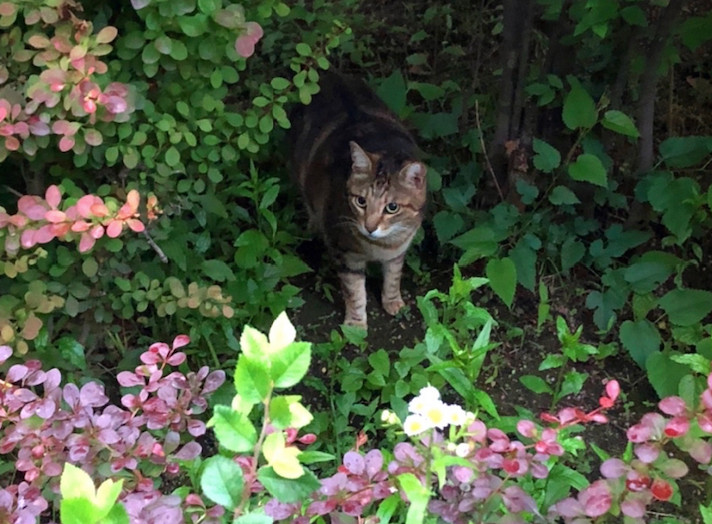
\includegraphics[width=0.8\linewidth]{figures/cat_momo_2.jpg}
\caption{\label{fig:cat2}This cat picture is located at the 'figures' folder.}
\end{figure}

\lipsum[14]

\subsection{Appendix subsection title here}
\lipsum[15]

\end{appendices}


\end{document}